\documentclass[11pt,a4paper]{article}

\usepackage[utf8]{inputenc}
\usepackage[T1]{fontenc}
\usepackage{amsmath,amssymb,amsfonts}
\usepackage{physics}
\usepackage{hyperref}
\usepackage{booktabs}
\usepackage{geometry}
\usepackage{enumitem}
\usepackage{listings}
\usepackage{xcolor}
\usepackage{graphicx}
\usepackage{subcaption}

\geometry{margin=1in}
\hypersetup{colorlinks=true, linkcolor=blue, urlcolor=blue, citecolor=blue}
\graphicspath{{../../output/woloshyn/}}

\lstset{
  language=Python,
  basicstyle=\ttfamily\small,
  keywordstyle=\color{blue},
  commentstyle=\color{gray},
  stringstyle=\color{red!70!black},
  showstringspaces=false,
  frame=single,
  breaklines=true,
}

\title{Derivation and Implementation Notes\\
\large Woloshyn --- Demonstrating Quantum Computing with the Quark Model\\
\normalsize arXiv:2301.10828v2}

\author{Companion document for the \texttt{quarksim} codebase}
\date{}

\begin{document}
\maketitle

\tableofcontents
\newpage

%=============================================================================
\section{The Physics Problem}
%=============================================================================

\subsection{Charmonium with Spin-Dependent Interactions}

This paper extends the quantum computing approach to charmonium by including \textbf{spin-dependent interactions}, which break the degeneracy between spin-singlet and spin-triplet states. Three channels are studied:
\begin{itemize}[nosep]
  \item ${}^1S_0$ (\textbf{$\eta_c$}): orbital $l=0$, spin singlet ($\vec{S}_c \cdot \vec{S}_{\bar{c}} = -3/4$)
  \item ${}^3S_1$ (\textbf{$J/\psi$}): orbital $l=0$, spin triplet ($\vec{S}_c \cdot \vec{S}_{\bar{c}} = +1/4$)
  \item ${}^1P_1$ (\textbf{$h_c$}): orbital $l=1$, spin singlet
\end{itemize}

\subsection{The Cornell Potential with Spin Contact Term}

The potential between the charm quark and anti-charm quark is:
\begin{equation}
  V(r) = -\frac{a}{r} + b\,r + V_s(r)\,\vec{S}_c \cdot \vec{S}_{\bar{c}}
  \label{eq:cornell}
\end{equation}
where $a = 4\alpha_s/3$ is the color Coulomb coupling, $b$ is the string tension, and $V_s(r)$ is the spin-dependent contact potential:
\begin{equation}
  V_s(r) = \frac{32\pi\alpha_s}{9\,m_c^2}\,\delta(r)
  \label{eq:spin_contact}
\end{equation}
The delta function is smeared with a Gaussian:
\begin{equation}
  \delta(r) = \left(\frac{\sigma}{\sqrt{\pi}}\right)^3 e^{-\sigma^2 r^2}
\end{equation}
Note that spin-orbit and tensor interactions are omitted as they are not relevant for the states considered here.

\textbf{Contrast with Gallimore:} The Gallimore implementation uses a spin-averaged potential ($V = -\kappa/r + \sigma r$) and considers only spin-averaged $S$-wave states. Woloshyn's inclusion of the contact term enables the study of the physical mass splitting between $\eta_c$ (2982~MeV) and $J/\psi$ (3097~MeV), a difference of 115~MeV.

\subsection{Parameters}

The parameters from Barnes \textit{et al.} (Table~1 of the paper):
\begin{center}
\begin{tabular}{lll}
\toprule
Symbol & Value & Description \\
\midrule
$\alpha_s$ & 0.5461 & Strong coupling constant \\
$b$ & 0.1425~GeV$^2$ & String tension \\
$m_c$ & 1.4794~GeV & Charm quark mass \\
$\sigma$ & 1.0946~GeV & Gaussian smearing parameter \\
$\omega$ & 1.2~fm$^{-1}$ & HO frequency (chosen from Fig.~1) \\
\bottomrule
\end{tabular}
\end{center}

\textbf{Units:} Unlike Gallimore (which works in MeV), all energies here are in fm$^{-1}$. The conversion factor is $\hbar c = 197.326$~MeV$\cdot$fm, so $1~\text{fm}^{-1} = 197.3$~MeV. The meson mass is $M = E + 2m_c$, where $E$ is the energy eigenvalue.

\vspace{0.3em}
\noindent\textbf{Code:} \texttt{hamiltonian.py}, constants in \texttt{CHARMONIUM\_PARAMS}.


%=============================================================================
\section{Harmonic Oscillator Basis}
%=============================================================================

\subsection{Basis States}

The Hamiltonian for the 3D harmonic oscillator is (Eq.~2):
\begin{equation}
  H_{\text{HO}} = -\frac{\vec{\nabla}^2}{2\mu} + \frac{1}{2}\mu\omega^2 r^2
  \label{eq:hho}
\end{equation}
The quark model Hamiltonian is rewritten as (Eq.~3):
\begin{equation}
  H_{\text{qm}} = H_{\text{HO}} + V(r) - \frac{1}{2}\mu\omega^2 r^2
  \label{eq:hqm}
\end{equation}
This decomposition is convenient because the matrix elements of $H_{\text{HO}}$ are trivially diagonal, and $V(r) - \frac{1}{2}\mu\omega^2 r^2$ contains the ``residual'' interaction.

The HO basis wavefunctions (unnormalized) are:
\begin{equation}
  r^l \, e^{-\frac{1}{2}\nu r^2} \, L_n^{l+1/2}(\nu r^2) \, Y_{lm}(\theta,\phi)
\end{equation}
where $\nu = \mu\omega$, $L_n^{l+1/2}$ is a generalized Laguerre polynomial, and the eigenenergy is $\omega(2n + l + 3/2)$ with $\hbar = 1$.

\subsection{Truncation to $N=4$ States}

The basis is truncated to $N=4$ radial states ($n = 0, 1, 2, 3$) for each channel. This gives a $4 \times 4$ Hamiltonian matrix encodable in \textbf{2 qubits} --- half the qubits needed for Gallimore's 3-orbital system.

The oscillator parameter $\omega = 1.2$~fm$^{-1}$ is chosen as a compromise: small $\omega$ gives better convergence for low-lying states (closer to the exact Schr\"odinger solution) but worse for higher states. The paper's Fig.~1 shows the eigenvalues vs.\ $\omega$, demonstrating the variational nature of the truncation.

\vspace{0.3em}
\noindent\textbf{Code:} The matrix is built in \texttt{hamiltonian.get\_matrix(channel)} using the paper's explicit matrices, or computed from scratch via \texttt{hamiltonian.compute\_matrix(channel)}.


%=============================================================================
\section{Matrix Elements}
%=============================================================================

\subsection{Structure}

The matrix elements of $H_{\text{qm}}$ in the HO basis are:
\begin{equation}
  \mel{m}{H_{\text{qm}}}{n} = \omega\!\left(2n + l + \tfrac{3}{2}\right)\delta_{mn}
    + \mel{m}{V(r) - \tfrac{1}{2}\mu\omega^2 r^2}{n}
\end{equation}

The first term is the diagonal HO eigenvalue. The second term contains:
\begin{itemize}[nosep]
  \item $-a\mel{m}{r^{-1}}{n}$: Coulomb integral (hypergeometric functions, same as Gallimore)
  \item $b\mel{m}{r}{n}$: Linear confinement integral (hypergeometric functions)
  \item $-\frac{1}{2}\mu\omega^2\mel{m}{r^2}{n}$: HO potential subtraction (tridiagonal, closed form)
  \item $V_s \cdot S \cdot S \cdot \mel{m}{\delta(r)}{n}$: Spin contact integral (numerical quadrature, $S$-waves only)
\end{itemize}

\subsection{Explicit Matrices}

The ${}^1S_0$ Hamiltonian matrix at $\omega = 1.2$~fm$^{-1}$ (Eq.~4):
\begin{equation}
  H_{{}^1S_0} = \begin{pmatrix}
    0.9431 & -0.8733 & -0.7690 & -0.5601 \\
    -0.8733 & 3.3365 & -0.5646 & -0.8648 \\
    -0.7690 & -0.5646 & 5.4382 & -0.1566 \\
    -0.5601 & -0.8648 & -0.1566 & 7.3451
  \end{pmatrix}
  \label{eq:h1s0}
\end{equation}

The ${}^3S_1$ matrix (Eq.~15 in the Appendix):
\begin{equation}
  H_{{}^3S_1} = \begin{pmatrix}
    1.0946 & -0.7114 & -0.6111 & -0.4112 \\
    -0.7114 & 3.5406 & -0.3910 & -0.6989 \\
    -0.6111 & -0.3910 & 5.6122 & -0.0119 \\
    -0.4112 & -0.6989 & -0.0119 & 7.5104
  \end{pmatrix}
  \label{eq:h3s1}
\end{equation}

The difference between ${}^1S_0$ and ${}^3S_1$ on the diagonal is due to the spin contact interaction: $\Delta H_{nn} = V_s \cdot [\tfrac{1}{4} - (-\tfrac{3}{4})] \cdot \mel{n}{\delta(r)}{n}$. For $n=0$: $\Delta = 1.0946 - 0.9431 = 0.1515$~fm$^{-1}$, corresponding to 30~MeV of hyperfine splitting per level.

\subsection{Eigenvalues (Table 3)}

\begin{center}
\begin{tabular}{l c c c}
\toprule
State & ${}^1S_0$ (fm$^{-1}$) & ${}^3S_1$ (fm$^{-1}$) & ${}^1P_1$ (fm$^{-1}$) \\
\midrule
1 & 0.395 & 0.753 & 2.783 \\
2 & 3.506 & 3.634 & 4.875 \\
3 & 5.664 & 5.723 & 6.765 \\
4 & 7.546 & 7.648 & 8.767 \\
\bottomrule
\end{tabular}
\end{center}

These are the target values for the VQITE algorithm.

\vspace{0.3em}
\noindent\textbf{Code:} Eigenvalues via \texttt{numpy.linalg.eigvalsh(get\_matrix(channel))}.


%=============================================================================
\section{Hamiltonian in Pauli Form (2 Qubits)}
%=============================================================================

\subsection{Direct Encoding}

With 4 basis states encoded in 2 qubits, the mapping is direct:
\begin{align}
  \ket{00} &\leftrightarrow \text{HO state } n=0 \nonumber\\
  \ket{01} &\leftrightarrow \text{HO state } n=1 \nonumber\\
  \ket{10} &\leftrightarrow \text{HO state } n=2 \nonumber\\
  \ket{11} &\leftrightarrow \text{HO state } n=3 \nonumber
\end{align}

\textbf{Key difference from Gallimore:} In the Jordan-Wigner encoding (3 qubits), only 3 of the $2^3 = 8$ computational basis states are physical (the 1-particle sector). Here, \emph{all} $2^2 = 4$ states are physical. This means:
\begin{itemize}[nosep]
  \item No need to project onto a physical subspace.
  \item The full $4 \times 4$ Pauli matrix equals the physical Hamiltonian directly.
  \item Fewer qubits (2 vs.\ 3) for more basis states (4 vs.\ 3).
\end{itemize}

\subsection{Pauli Decomposition}

A general $4 \times 4$ real symmetric matrix decomposes into 10 Pauli terms (the 6 imaginary operators $XY, YX, ZY, YZ, IY, YI$ vanish for real matrices):
\begin{equation}
  H = c_0\,II + c_1\,Z_0 + c_2\,Z_1 + c_3\,Z_0 Z_1 + c_4\,X_0 + c_5\,X_1
    + c_6\,Z_0 X_1 + c_7\,X_0 Z_1 + c_8\,X_0 X_1 + c_9\,Y_0 Y_1
  \label{eq:pauli_form}
\end{equation}

The coefficients are computed as:
\begin{equation}
  c_k = \frac{1}{4}\text{Tr}(H \cdot P_k)
\end{equation}

\subsection{Pauli Coefficients}

\begin{center}
\begin{tabular}{l r r r}
\toprule
Term & ${}^1S_0$ & ${}^3S_1$ & ${}^1P_1$ \\
\midrule
$c_0$ (II) & 4.273 & 4.439 & 5.798 \\
$c_1$ ($Z_0$) & $-2.119$ & $-2.122$ & $-1.910$ \\
$c_2$ ($Z_1$) & $-1.082$ & $-1.086$ & $-0.964$ \\
$c_3$ ($Z_0 Z_1$) & $-0.129$ & $-0.137$ & $-0.067$ \\
$c_4$ ($X_0$) & $-0.817$ & $-0.655$ & $-0.446$ \\
$c_5$ ($X_1$) & $-0.515$ & $-0.350$ & 0.083 \\
$c_6$ ($Z_0 X_1$) & $-0.358$ & $-0.361$ & $-0.323$ \\
$c_7$ ($X_0 Z_1$) & 0.048 & 0.044 & $-0.064$ \\
$c_8$ ($X_0 X_1$) & $-0.562$ & $-0.401$ & $-0.095$ \\
$c_9$ ($Y_0 Y_1$) & $-0.002$ & 0.010 & 0.133 \\
\bottomrule
\end{tabular}
\end{center}

\textbf{Note on qubit ordering:} The paper uses PennyLane (big-endian: qubit~0 = MSB), while our Qiskit implementation uses little-endian (qubit~0 = LSB). The paper's $Z_0$ corresponds to Qiskit's \texttt{'ZI'}, and $Z_1$ to \texttt{'IZ'}. The coefficients are physically identical; only the labeling convention differs.

\vspace{0.3em}
\noindent\textbf{Code:} \texttt{hamiltonian.build\_pauli\_hamiltonian(channel)} decomposes via \texttt{matrix\_to\_pauli(H)}. Validation via \texttt{validate\_pauli\_hamiltonian()} confirms the $4\times 4$ Pauli matrix reconstructs the original matrix exactly.


%=============================================================================
\section{Variational Quantum Imaginary Time Evolution}
%=============================================================================

\subsection{Imaginary Time Evolution}

For a Hamiltonian $H$ with eigenvalues $\{\lambda_i\}$ and eigenstates $\{\ket{\phi_i}\}$, the imaginary time evolution of an initial state $\ket{\psi_0}$ is (Eq.~5):
\begin{equation}
  e^{-H\tau}\ket{\psi_0} = \sum_i e^{-\lambda_i \tau} \braket{\phi_i|\psi_0}\ket{\phi_i}
  \label{eq:ite}
\end{equation}
For large $\tau$, the lowest-energy component dominates. However, this operation is \textbf{non-unitary} and cannot be directly implemented on a quantum computer.

\subsection{The Variational Approach}

We parametrize the state as $\ket{\psi(\vec{\theta})} = U(\vec{\theta})\ket{0}$ and seek unitary updates that approximate imaginary time evolution. The variational principle (Eqs.~7--8) leads to the evolution equation (Eq.~9):
\begin{equation}
  \boxed{\sum_j A_{ij}\,\dot{\theta}_j = C_i}
  \label{eq:vqite_update}
\end{equation}
where:
\begin{align}
  C_i &= -\frac{\partial E_\tau}{\partial \theta_i}
    \label{eq:gradient} \\
  A_{ij} &= -\frac{\partial^2 \braket{\psi(\tilde{\theta})|\psi(\vec{\theta})}}{\partial\theta_i\,\partial\theta_j}
    \label{eq:metric}
\end{align}

Here $E_\tau = \mel{\psi(\vec{\theta}(\tau))}{H}{\psi(\vec{\theta}(\tau))}$ is the energy, and the derivative in \eqref{eq:metric} acts only on the ket (right side). The matrix $A$ is the \textbf{quantum metric tensor} (Fubini-Study metric), which captures the geometry of the parameter space.

Parameters are updated as:
\begin{equation}
  \vec{\theta}(\tau + \Delta\tau) = \vec{\theta}(\tau) + \Delta\tau\,\dot{\vec{\theta}}
\end{equation}
where $\Delta\tau$ acts as a learning rate.

\subsection{The Ansatz Circuit (Fig.~2)}

The variational ansatz uses 3 parameters on 2 qubits:
\begin{center}
\begin{tabular}{l}
\texttt{q0: --Ry($\theta_0$)--*-----------} \\
\texttt{~~~~~~~~~~~~~~~~~~|} \\
\texttt{q1: --Ry($\theta_1$)--X--Ry($\theta_2$)--}
\end{tabular}
\end{center}

With 3 parameters, this circuit can produce any real superposition of 4 basis states (3 free parameters = 4 real amplitudes $-$ 1 normalization $-$ 0 phases since all are real).

Starting from $\ket{00}$:
\begin{align}
  \ket{\psi(\theta_0,\theta_1,\theta_2)} &= \cos\!\tfrac{\theta_0}{2}\left(\cos\!\tfrac{\theta_1+\theta_2}{2}\ket{00} + \sin\!\tfrac{\theta_1+\theta_2}{2}\ket{10}\right) \nonumber\\
    &\quad + \sin\!\tfrac{\theta_0}{2}\left(\sin\!\tfrac{\theta_1-\theta_2}{2}\ket{01} + \cos\!\tfrac{\theta_1-\theta_2}{2}\ket{11}\right)
\end{align}
(Note: state indices use Qiskit's $\ket{q_1\,q_0}$ ordering.)

\subsection{Computing $C_i$ and $A_{ij}$}

\textbf{Energy gradient} $C_i$: We use the \textbf{parameter-shift rule} for $RY$ gates:
\begin{equation}
  \frac{\partial E}{\partial \theta_k} = \frac{E(\theta_k + \pi/2) - E(\theta_k - \pi/2)}{2}
\end{equation}
This is exact (not a finite-difference approximation) because $RY(\theta) = e^{-i\theta Y/2}$ generates a sinusoidal parameter dependence.

\textbf{Metric tensor} $A_{ij}$: We use \textbf{finite differences} on the overlap function $f(\vec{\theta}) = \braket{\psi_0|\psi(\vec{\theta})}$:
\begin{equation}
  A_{ij} \approx -\frac{f(\vec{\theta}+\varepsilon\hat{e}_i+\varepsilon\hat{e}_j) - f(\vec{\theta}+\varepsilon\hat{e}_i-\varepsilon\hat{e}_j) - f(\vec{\theta}-\varepsilon\hat{e}_i+\varepsilon\hat{e}_j) + f(\vec{\theta}-\varepsilon\hat{e}_i-\varepsilon\hat{e}_j)}{4\varepsilon^2}
\end{equation}
with $\varepsilon = 10^{-4}$. The matrix $A$ is regularized as $A + \lambda I$ ($\lambda = 10^{-4}$) to handle near-singular cases when the state is close to a critical point in parameter space.

\subsection{Convergence}

\begin{figure}[h]
\centering
\begin{subfigure}[t]{0.48\textwidth}
  \centering
  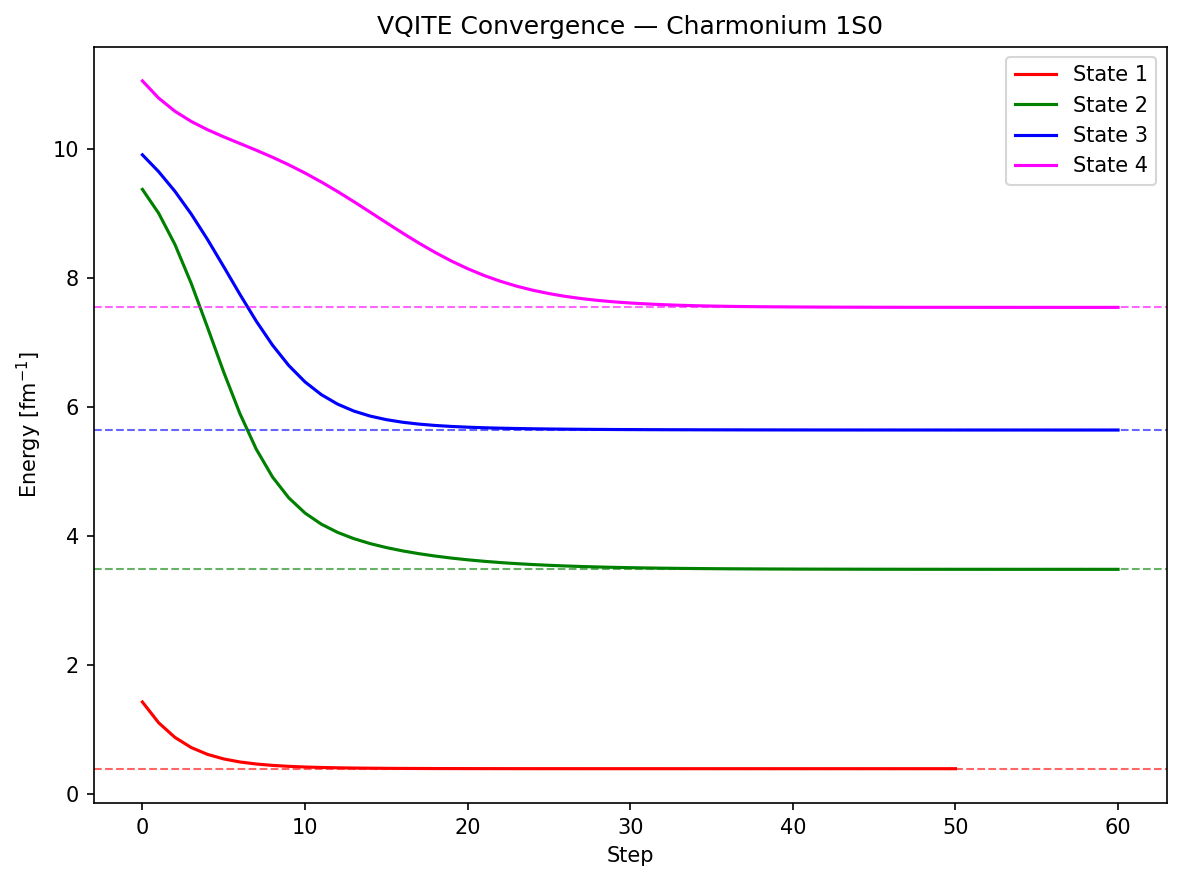
\includegraphics[width=\textwidth]{vqite_convergence_1S0.png}
  \caption{${}^1S_0$ channel}
\end{subfigure}
\hfill
\begin{subfigure}[t]{0.48\textwidth}
  \centering
  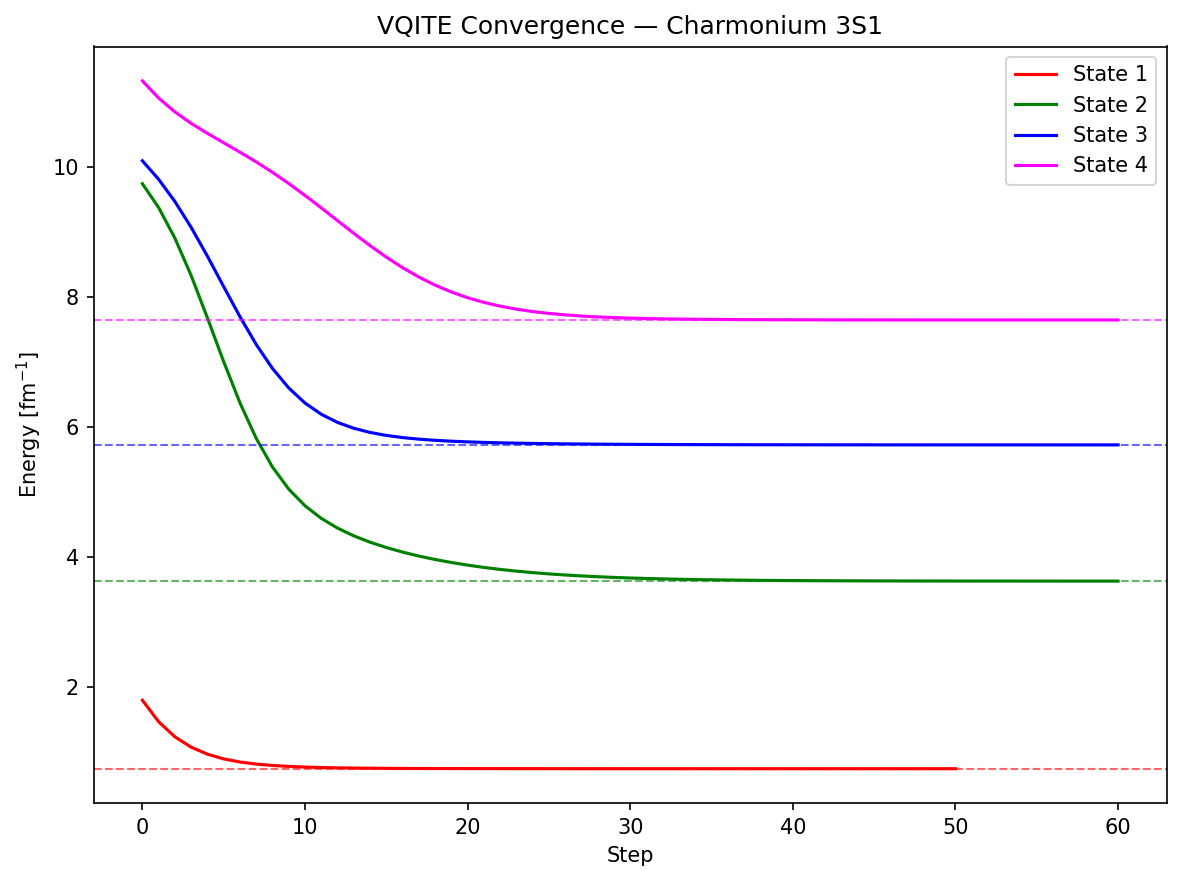
\includegraphics[width=\textwidth]{vqite_convergence_3S1.png}
  \caption{${}^3S_1$ channel}
\end{subfigure}

\vspace{0.5em}
\begin{subfigure}[t]{0.48\textwidth}
  \centering
  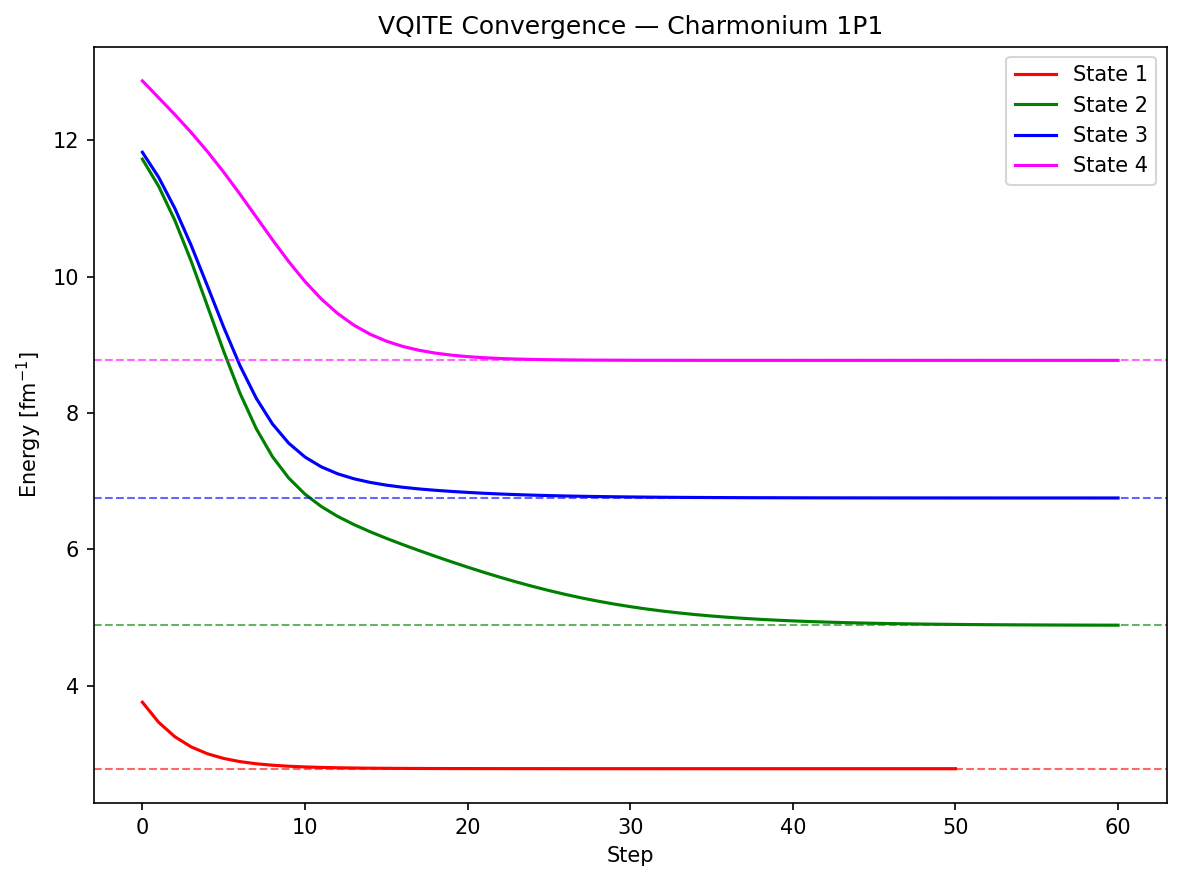
\includegraphics[width=\textwidth]{vqite_convergence_1P1.png}
  \caption{${}^1P_1$ channel}
\end{subfigure}
\caption{VQITE convergence for all three channels. Solid lines show the energy at each imaginary time step; horizontal dashed lines are the eigenvalues from diagonalizing the truncated Hamiltonian. Parameters: $\Delta\tau = 0.02$, initial $\theta_i = 0.5$, 50 steps. Compare with Figs.~4--6 of the paper.}
\label{fig:vqite_convergence}
\end{figure}

The ground state converges within $\sim$20--30 steps. Excited states (computed via the penalty method, Section~\ref{sec:excited}) take slightly longer.

\vspace{0.3em}
\noindent\textbf{Code:} \texttt{vqite.run\_vqite()} implements the full loop. \texttt{vqite.compute\_energy\_gradient()} and \texttt{vqite.compute\_metric\_tensor()} compute $C$ and $A$ respectively.


%=============================================================================
\section{Excited States}
\label{sec:excited}
%=============================================================================

\subsection{Penalty Method (Eq.~12)}

To find the $k$-th excited state, we add a penalty term to the energy that pushes the variational state away from all lower-lying states:
\begin{equation}
  E_{\text{eff}} = \mel{\psi(\vec{\theta})}{H}{\psi(\vec{\theta})} + \alpha \sum_{j < k} \left|\braket{\phi_j | \psi(\vec{\theta})}\right|^2
  \label{eq:penalty}
\end{equation}
where $\ket{\phi_j}$ are the previously determined eigenstates and $\alpha$ is a large positive coefficient.

\textbf{Contrast with Gallimore:} Gallimore uses an explicit orthogonalization in parameter space (reducing from 2 to 1 parameter for the first excited state). Woloshyn's penalty method is more general: it works for any number of excited states and any ansatz, at the cost of choosing $\alpha$ large enough.

In practice, $\alpha = 10$ works well for all channels. The overlap terms can be computed via the $U_i U_f^\dagger$ circuit (Fig.~3 of the paper) or directly from statevectors.

\subsection{Sequential Computation}

States are computed in order:
\begin{enumerate}[nosep]
  \item Ground state: VQITE with $H$
  \item 1st excited: VQITE with $H + \alpha|\braket{\phi_0|\cdot}|^2$
  \item 2nd excited: VQITE with $H + \alpha\left(|\braket{\phi_0|\cdot}|^2 + |\braket{\phi_1|\cdot}|^2\right)$
  \item 3rd excited: determined by the remaining orthogonal direction (or VQITE with 3 penalty terms)
\end{enumerate}

\vspace{0.3em}
\noindent\textbf{Code:} \texttt{vqite.run\_vqite\_excited()} takes a list of lower-state wavefunctions and adds the penalty.


%=============================================================================
\section{M1 Transition Amplitudes}
%=============================================================================

\subsection{Physics}

\textbf{M1 transitions} connect spin-singlet and spin-triplet states with the same orbital angular momentum (e.g., ${}^3S_1 \to {}^1S_0$). In the nonrelativistic limit, the transition involves a spin flip, and the spatial part of the amplitude is simply the wavefunction overlap:
\begin{equation}
  \mathcal{A}_{M1} = \braket{\psi_f | \psi_i}, \qquad |\mathcal{A}_{M1}|^2 = \text{squared amplitude}
\end{equation}

Because the spin-dependent interaction slightly distorts the spatial wavefunctions in different channels, the overlap is close to (but not exactly) 1 for corresponding states and close to 0 for non-corresponding states.

\subsection{Quantum Circuits}

\textbf{Overlap circuit (Fig.~3):} Prepare $\ket{\psi_i}$ then apply $U_f^\dagger$. Measuring $\ket{00}$ gives $P(00) = |\braket{\psi_f|\psi_i}|^2$.

\textbf{Swap test (Fig.~7):} Uses an ancilla qubit and controlled-SWAP. The measurement yields:
\begin{equation}
  P(\text{ancilla} = 0) = \frac{1 + |\braket{\psi_f|\psi_i}|^2}{2}
\end{equation}
This is less precise for small overlaps but doesn't require implementing $U^\dagger$.

\subsection{Results}

\begin{center}
\begin{tabular}{l c c}
\toprule
Transition & Paper (exact) & Our w.f.\ sim \\
\midrule
$1{}^3S_1 \to 1{}^1S_0$ & 0.9826 & 0.994 \\
$2{}^3S_1 \to 1{}^1S_0$ & 0.0107 & 0.004 \\
$2{}^3S_1 \to 2{}^1S_0$ & 0.9781 & 0.994 \\
$3{}^3S_1 \to 2{}^1S_0$ & 0.0061 & 0.002 \\
\bottomrule
\end{tabular}
\end{center}

The ``exact'' column uses solutions of the Schr\"odinger equation (Table~2 of the paper), while our results use the truncated basis. The dominant overlaps ($\sim 1$) match well; the small off-diagonal overlaps differ because they are sensitive to basis truncation.

\vspace{0.3em}
\noindent\textbf{Code:} \texttt{transitions.m1\_overlap()} for statevector computation. \texttt{transitions.build\_overlap\_circuit()} and \texttt{transitions.build\_swap\_test\_circuit()} for the quantum circuit versions.


%=============================================================================
\section{E1 Transition Amplitudes}
%=============================================================================

\subsection{Physics}

\textbf{E1 transitions} connect states with $\Delta L = 1$ (S-wave $\leftrightarrow$ P-wave) and the same spin. The transition amplitude is governed by the radial matrix element:
\begin{equation}
  \braket{u_f(r) | r | u_i(r)} = \int_0^\infty u_f(r)\, r\, u_i(r)\, dr
\end{equation}
where $u_f$ is a P-wave ($l=1$) state and $u_i$ is an S-wave ($l=0$) state.

\subsection{Matrix Elements of $r$ (Eq.~13)}

The matrix $\mel{m_P}{r}{n_S}$ connecting P-wave and S-wave HO basis states is (in fm):
\begin{equation}
  R = \begin{pmatrix}
    0.578 & -0.472 & 0 & 0 \\
    0 & 0.746 & -0.667 & 0 \\
    0 & 0 & 0.882 & -0.817 \\
    0 & 0 & 0 & 1.000
  \end{pmatrix}
\end{equation}

The tridiagonal structure reflects the selection rule: HO states only couple to adjacent radial quantum numbers via $r$.

\subsection{Pauli Decomposition (Eq.~14)}

The $r$-operator matrix has \textbf{complex Pauli coefficients} (unlike the Hamiltonian which is real symmetric). The decomposition includes $Y$ terms:
\begin{equation}
  \hat{r} = c_0 + c_1 Z_0 + c_2 Z_1 + c_3 Z_0 Z_1 + c_4(X_0 X_1 + Y_0 Y_1)
    + c_5(X_1 - iY_1) + c_6 Z_0(X_1 + iY_1) + c_7(X_0 Y_1 - Y_0 X_1)
\end{equation}

\subsection{Hadamard Test (Fig.~8)}

The Hadamard test circuit computes $\braket{\psi_f|\hat{O}|\psi_i}$ for an arbitrary operator $\hat{O}$. It uses an ancilla qubit, controlled state preparations, and a rotation $R$ to select the real or imaginary part:
\begin{itemize}[nosep]
  \item $R = R_y(-\pi/2)$: ancilla measurement gives $\braket{\sigma_x} = 2\,\text{Re}\braket{\psi_f|\hat{O}|\psi_i}$
  \item $R = R_x(\pi/2)$: ancilla measurement gives $\braket{\sigma_y} = 2\,\text{Im}\braket{\psi_f|\hat{O}|\psi_i}$
\end{itemize}

\vspace{0.3em}
\noindent\textbf{Code:} \texttt{transitions.e1\_matrix\_elements()} computes $R$. \texttt{transitions.e1\_amplitude()} does statevector computation. \texttt{transitions.build\_hadamard\_test\_circuit()} builds the circuit.


%=============================================================================
\section{Readout Error Mitigation}
%=============================================================================

\subsection{The Problem}

On real quantum hardware, qubits may be misidentified during measurement: $\ket{0}$ read as $\ket{1}$ and vice versa. For $n$ qubits, the readout error is characterized by a $2^n \times 2^n$ calibration matrix $M$:
\begin{equation}
  \vec{p}_{\text{noisy}} = M \cdot \vec{p}_{\text{ideal}}
\end{equation}
where $\vec{p}$ is the vector of measurement probabilities.

\subsection{Mitigation Strategy}

The mitigation procedure (described in the paper's Section~5):
\begin{enumerate}[nosep]
  \item \textbf{Calibrate:} Prepare each computational basis state $\ket{00}, \ket{01}, \ket{10}, \ket{11}$ and measure. The resulting statistics form the columns of $M$.
  \item \textbf{Correct:} Apply $M^{-1}$ to the measured probability vector to recover the ideal distribution.
\end{enumerate}

For 2 qubits, $M$ is only $4 \times 4$, making inversion straightforward. The paper uses the IBM \texttt{ibmq\_manila} noise model for demonstration.

\subsection{Effect on Results}

The readout error mitigation is most impactful for:
\begin{itemize}[nosep]
  \item \textbf{Energy calculations}: Figs.~9--11 show ideal vs.\ noisy vs.\ mitigated VQITE convergence. Mitigation brings noisy results close to ideal.
  \item \textbf{M1 overlaps}: Table~6 shows that large overlaps ($\sim 1$) are well-recovered, but small overlaps ($\sim 0.001$) remain unreliable even after mitigation.
\end{itemize}


%=============================================================================
\section{Results Summary}
%=============================================================================

\subsection{Energy Levels}

Our VQITE simulation reproduces the paper's eigenvalues (Table~3) to within the truncation error:

\begin{center}
\begin{tabular}{l c c c c}
\toprule
& \multicolumn{2}{c}{${}^1S_0$} & \multicolumn{2}{c}{${}^3S_1$} \\
State & VQITE & Paper & VQITE & Paper \\
\midrule
1 & 0.391 & 0.395 & 0.752 & 0.753 \\
2 & 3.483 & 3.506 & 3.633 & 3.634 \\
3 & 5.643 & 5.664 & 5.727 & 5.723 \\
4 & 7.545 & 7.546 & 7.646 & 7.648 \\
\bottomrule
\end{tabular}
\end{center}

\begin{figure}[h]
\centering
\begin{subfigure}[t]{0.32\textwidth}
  \centering
  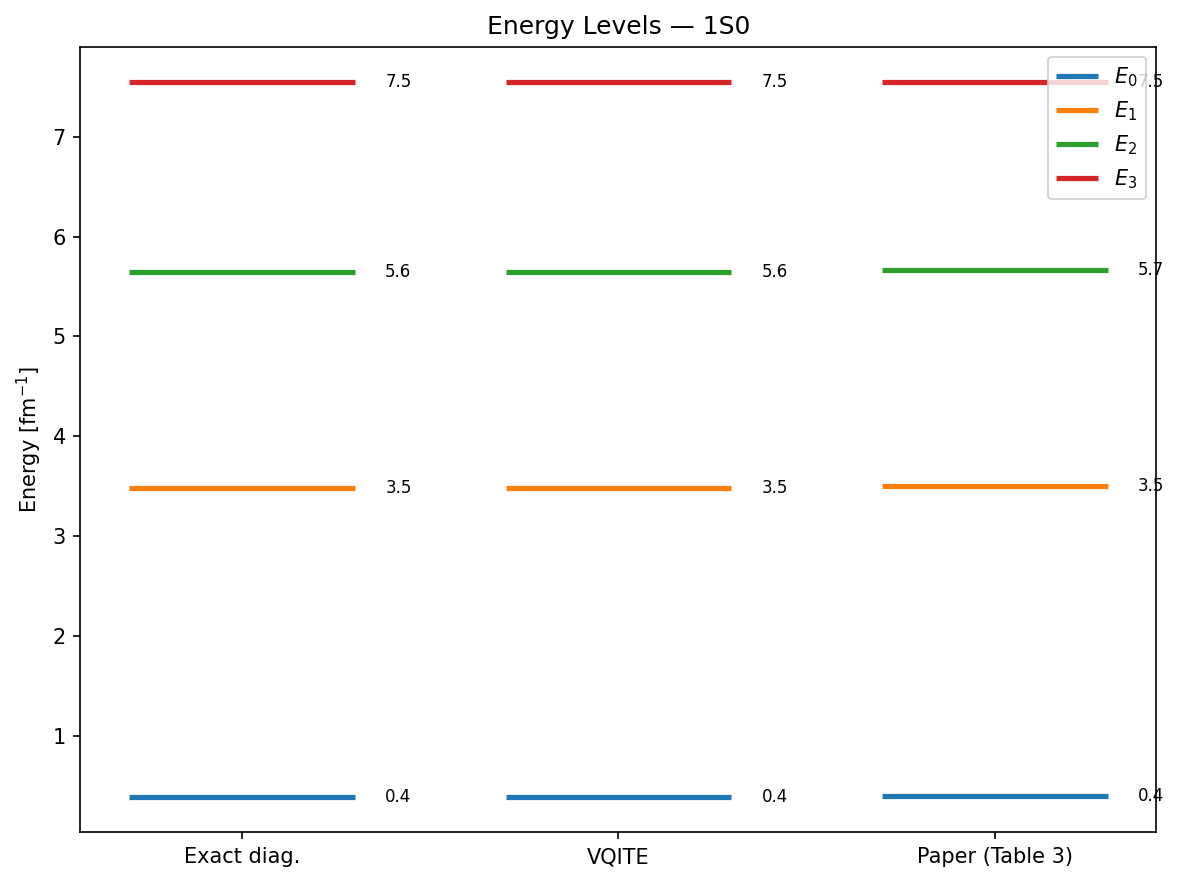
\includegraphics[width=\textwidth]{energy_levels_1S0.png}
  \caption{${}^1S_0$}
\end{subfigure}
\hfill
\begin{subfigure}[t]{0.32\textwidth}
  \centering
  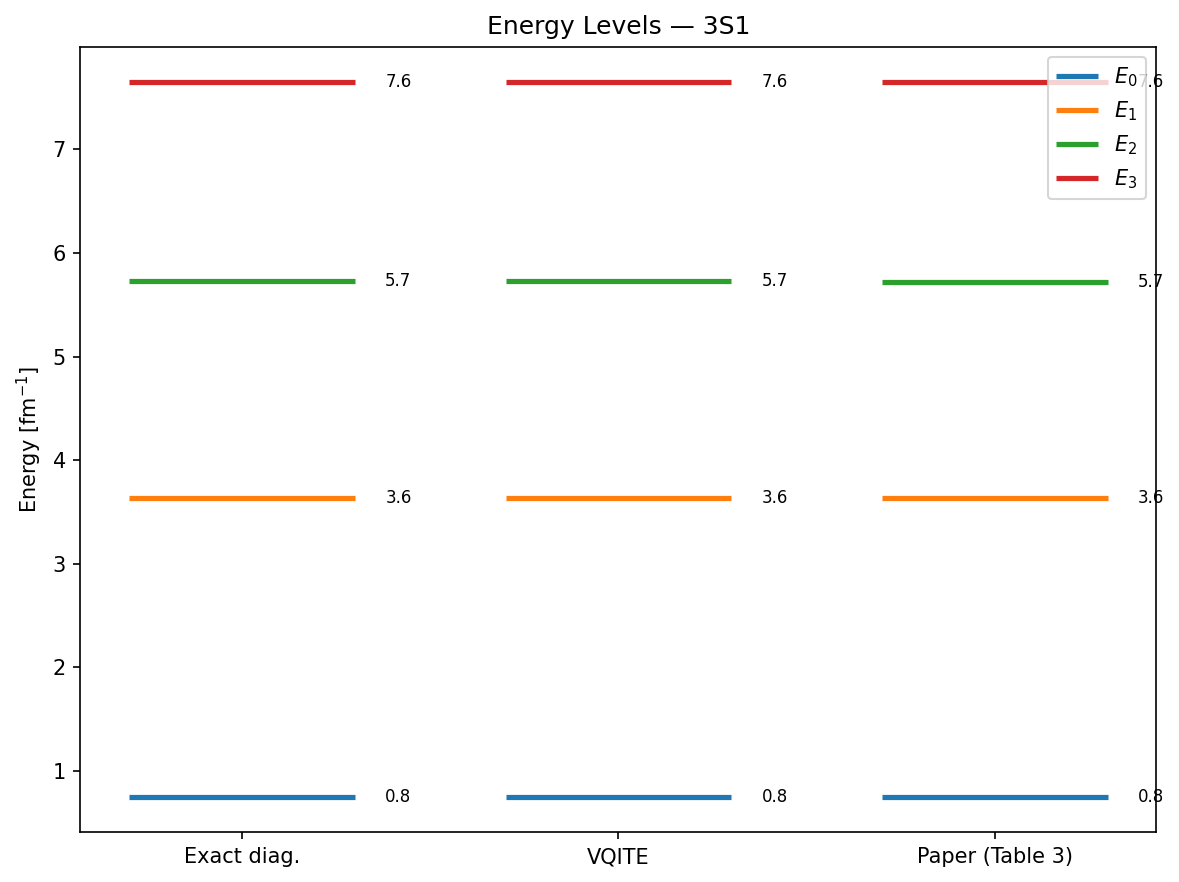
\includegraphics[width=\textwidth]{energy_levels_3S1.png}
  \caption{${}^3S_1$}
\end{subfigure}
\hfill
\begin{subfigure}[t]{0.32\textwidth}
  \centering
  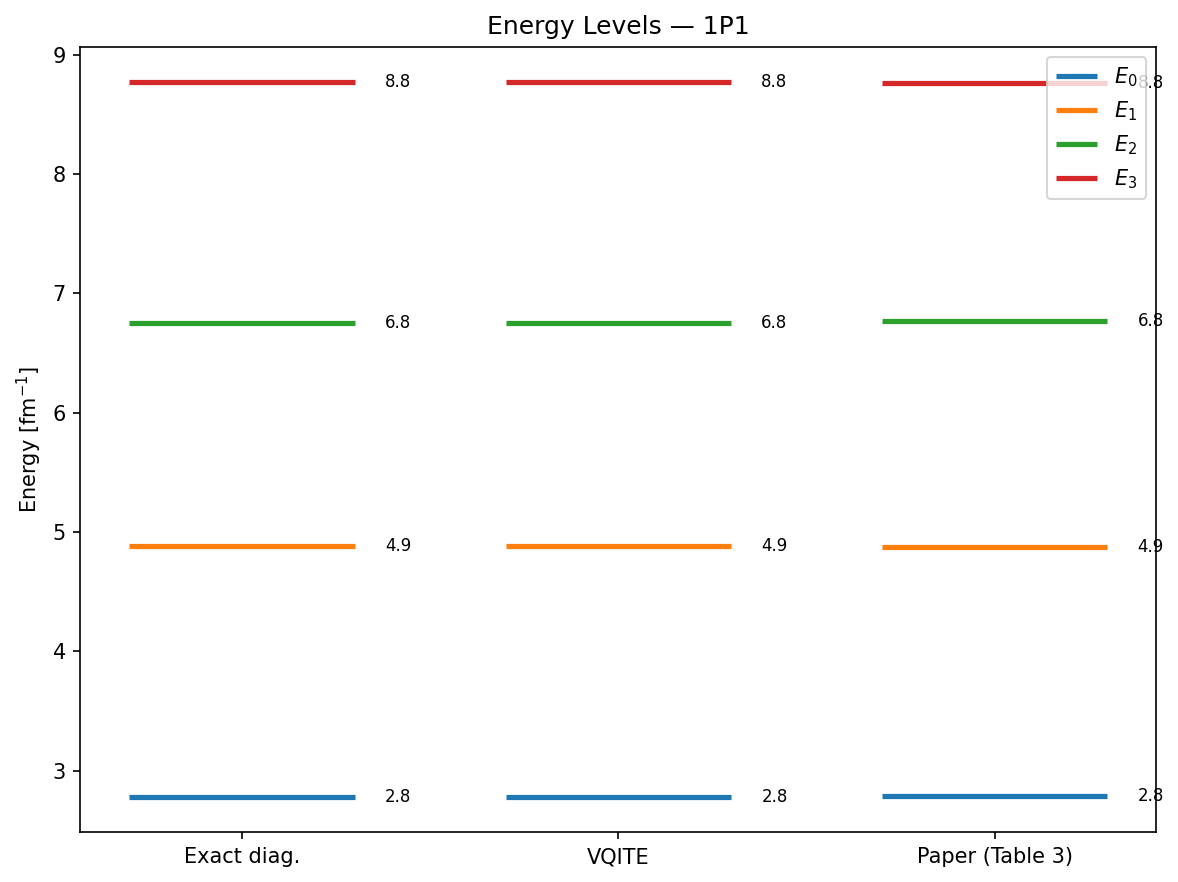
\includegraphics[width=\textwidth]{energy_levels_1P1.png}
  \caption{${}^1P_1$}
\end{subfigure}
\caption{Energy level comparison: VQITE results vs.\ exact diagonalization vs.\ paper's Table~3 values.}
\label{fig:energy_levels}
\end{figure}


%=============================================================================
\section{Code--Equation Mapping}
%=============================================================================

\begin{center}
\begin{tabular}{lll}
\toprule
Paper reference & Code location & Description \\
\midrule
Eq.~(1): Schr\"odinger eq. & \texttt{hamiltonian.compute\_matrix()} & From-scratch computation \\
Eq.~(3): $H_{\text{qm}}$ & \texttt{hamiltonian.get\_matrix()} & Paper's explicit matrices \\
Eq.~(4): ${}^1S_0$ matrix & \texttt{PAPER\_MATRICES["1S0"]} & Hardcoded constant \\
Section~2.2.1: Pauli form & \texttt{hamiltonian.matrix\_to\_pauli()} & $c_k = \text{Tr}(HP_k)/4$ \\
Fig.~2: Ansatz circuit & \texttt{ansatz.build\_ansatz()} & 3-param Ry+CNOT \\
Eq.~(9): VQITE update & \texttt{vqite.run\_vqite()} & Full evolution loop \\
Eq.~(10): Gradient $C_i$ & \texttt{vqite.compute\_energy\_gradient()} & Parameter-shift rule \\
Eq.~(11): Metric $A_{ij}$ & \texttt{vqite.compute\_metric\_tensor()} & Finite differences \\
Eq.~(12): Excited penalty & \texttt{vqite.run\_vqite\_excited()} & $E + \alpha|\braket{\phi|\psi}|^2$ \\
Eq.~(13): $\mel{m_P}{r}{n_S}$ & \texttt{transitions.e1\_matrix\_elements()} & Numerical integration \\
Eq.~(14): $r$ in Pauli form & \texttt{transitions.build\_e1\_pauli\_operator()} & Complex coefficients \\
Fig.~3: Overlap circuit & \texttt{transitions.build\_overlap\_circuit()} & $U_i U_f^\dagger$ \\
Fig.~7: Swap test & \texttt{transitions.build\_swap\_test\_circuit()} & Ancilla + CSWAP \\
Fig.~8: Hadamard test & \texttt{transitions.build\_hadamard\_test\_circuit()} & $\braket{\psi_f|O|\psi_i}$ \\
\bottomrule
\end{tabular}
\end{center}


%=============================================================================
\section{Running the Simulation}
%=============================================================================

\begin{lstlisting}[language=bash]
# Install
uv venv && source .venv/bin/activate
uv pip install -e .

# Run all channels
python -m quarksim.woloshyn.run --channel all --transitions

# Single channel, custom parameters
python -m quarksim.woloshyn.run --channel 1S0 --n-steps 80 --dtau 0.01

# Output directory
python -m quarksim.woloshyn.run --output results/woloshyn
\end{lstlisting}

\textbf{Output files:}
\begin{itemize}[nosep]
  \item \texttt{vqite\_result\_\{channel\}.json} --- full simulation record per channel
  \item \texttt{vqite\_convergence\_\{channel\}.png} --- energy vs.\ step (Fig.~\ref{fig:vqite_convergence})
  \item \texttt{energy\_levels\_\{channel\}.png} --- level comparison (Fig.~\ref{fig:energy_levels})
  \item \texttt{wavefunction\_\{channel\}.png} --- ground state amplitudes
\end{itemize}

\end{document}
